\chapter{Navigation of timed transcripts}

\section{Evaluation}

\subsection{System design}
The interface for the system has heavily inspired by Hyperaudio Pad, an
open-source video editor that allows users to edit using timed transcripts. A
screenshot of the interface is shown in Figure~\ref{fig:hyperaudio-pad}. The
interface is divided into two columns -- the left displays the transcript of
the current video. Text can be selected and dragged to the right column to
create and mix video clips.

\begin{figure}[ht]
  \centering
  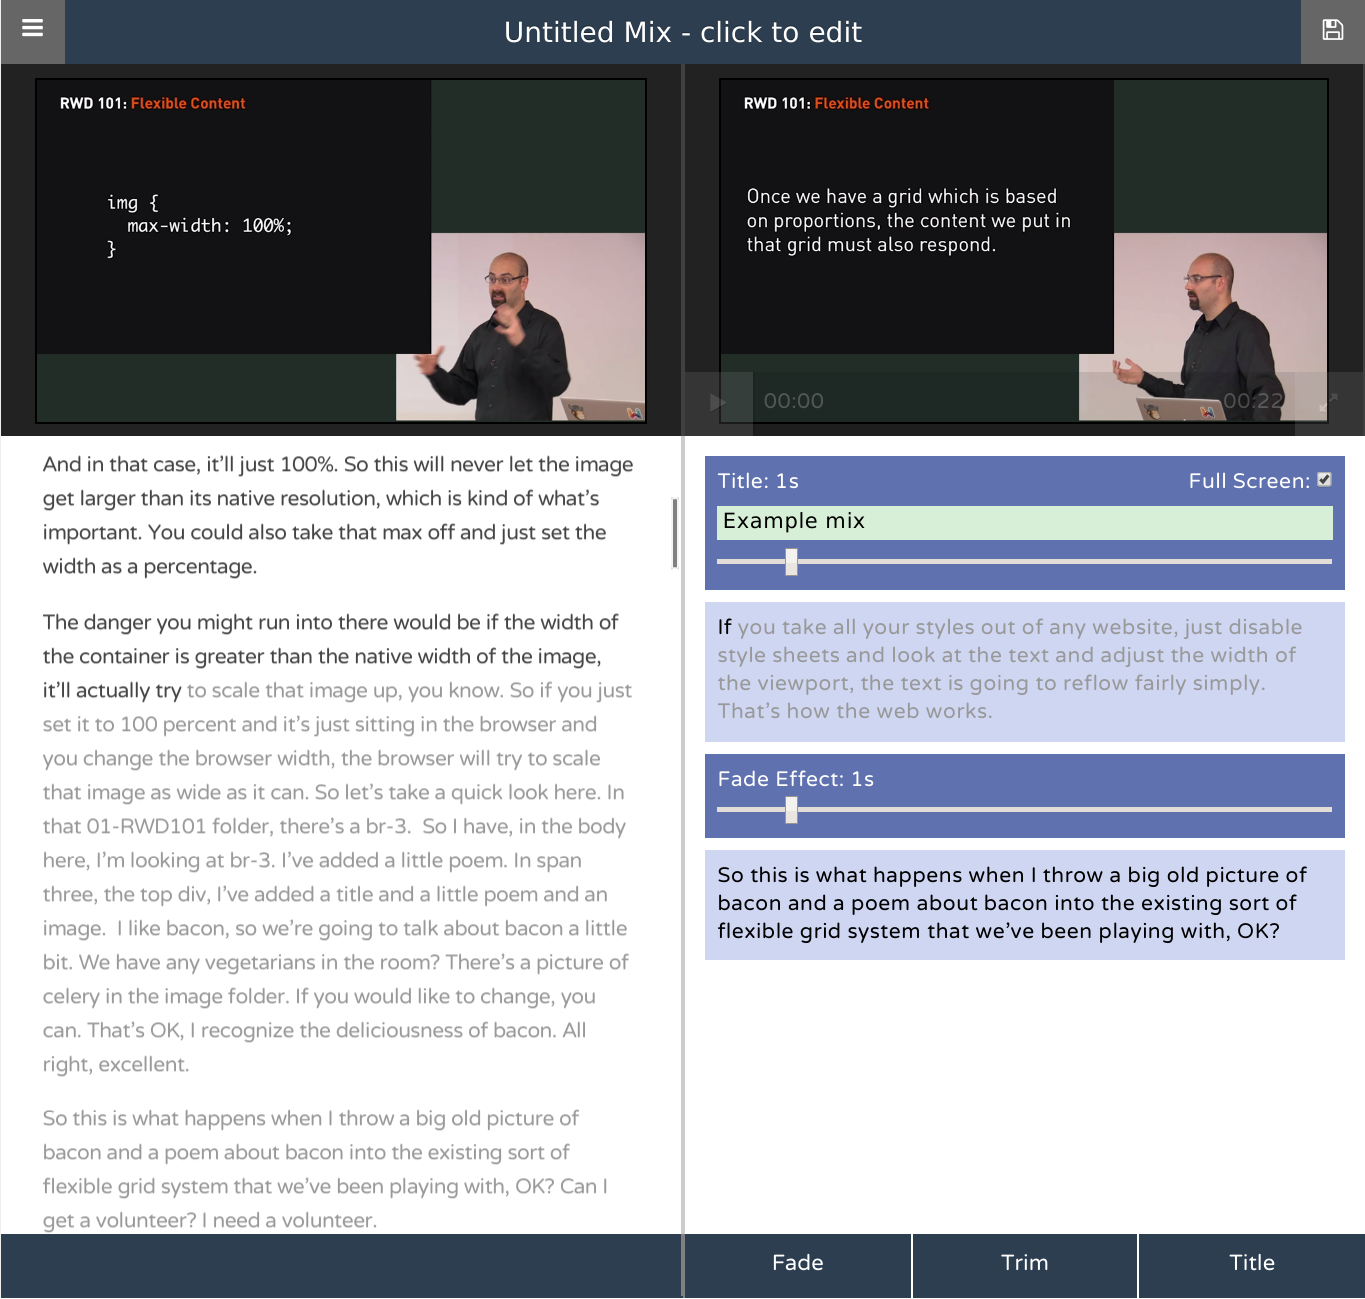
\includegraphics[width=0.6\textwidth]{figs/hyperaudio-pad-example.png}
  \caption{Hyperaudio Pad interface}
  \label{fig:hyperaudio-pad}
\end{figure}

\subsection{System features}
This section lists and describes the features of the prototype system developed
for the evaluation.

\subsubsection{User accounts}
Access to the system is managed through user accounts. Accounts can only be
created by the experimenter. User authentication is handled using the BBC iD
sign-in system\footnote{\url{http://www.bbc.co.uk/id/info}}.

\subsubsection{Projects}
Each user can create multiple projects in order to keep their work organised.

\subsubsection{Upload}
Users can upload their own audio recordings to the system.  Each recording can
be given a name to identify it. When uploading a recording, the user is
prompted to specify whether the accent of the speaker is British or American
(to assist the automatic speech recognition), and agree to a disclaimer about
the security of uploading content.

After upload, the recordings are converted to 16-bit 48kHz stereo WAV format,
an MP3 `scratch' version is created and the scratch version is sent to a
third-party speech-to-text service.

\subsubsection{Transcript alignment}
As part of the upload feature, the user can optionally upload a transcription
of the recording in .docx format. The text from the uploaded transcript is
considered to be a perfect verbatim transcription. The text is aligned to the
output of the speech-to-text system so that a timestamp is then attached to
each word of the uploaded transcript.

\subsubsection{Transcript display}
The transcript of the uploaded recording (either automatic or aligned) is
displayed to the user in the system interface. When the user clicks on a word,
the recording starts playing back from the time that word is spoken.

\subsubsection{Transcript editing}
The user can edit the recording's transcript by double-clicking on a word,
typing the new word and pressing \texttt{Enter}. Their changes can be saved by
pressing a Save button at the top of the transcript display.

\subsubsection{Waveform display}
An audio waveform is displayed at the top of the interface. The waveform
display is split into two rows. The bottom row displays the waveform from the
entire recording, from beginning to end. The top row displays a `zoomed-in'
subset of the bottom row, dependent on the current position of the playback.

\subsubsection{Clipping}
Users can create an audio clip by highlighting text in the transcript column on
the left, then dragging the highlighted text into the edit column on the right.
Clips from different recordings can be combined into a single edit.  The clips
in the edit column can be played, paused and stopped by the user.

\subsubsection{Clip re-ordering}
Clips in the edit column can be re-ordered by dragging them up or down. As
a clip is being dragged, the other clips move dynamically to make space for it.

\subsubsection{Copy}
The transcript and edit columns each have a `copy' button. This opens a dialog
with a text box of the transcript or edit text, with the text automatically
selected. The dialog explains to the user that they can copy the text by
pressing \texttt{Ctrl + C}.

\subsubsection{Print}
The transcript and edit columns each have a `print' button. This launches the
browser's print feature with the text of the transcript or edit. The user can
then continue the normal process of printing a document.

\subsubsection{Export}
The audio of the edit created by the user can be exported in a number of
different formats. The first is the uncompressed audio format WAV. This cuts
together the desired clips using the original recordings and concatenates them
into one recording. As the original recordings are used, the sound quality is
identical. However, the unselected bits of the recording are not exported,
meaning that the user can't easily readjust the edit points after exporting.

The other two formats are compatible with the BBC's two most popular DAWs --
SADiE and dira! Startrack. In each of these cases, the exported file includes
the full original recordings of each clip used, and an `edit decision list'
(EDL), which describes the in and out points of each edit. This means that the
user can use the DAW's interface to easily readjust edit points and add other
content such as music, presenter links and sound effects.

\subsection{System implementation}
The prototype system was created using modern web technologies. This approach
means that it can be accessed using the internet and is compatible with any
modern web browser on any computer platform. The abundance of well-supported
software libraries for these technologies also mean that development can be
done very quickly.

\subsubsection{Back-end}
The back-end of the system runs on a virtualised Ubuntu 14.04 server at BBC
R\&D. The NodeJS platform is used with the Express framework to run the web
services. MongoDB is used as a database for storing user information and the
metadata of recordings, projects and edits. Uploaded audio is processed using
FFmpeg, then sent to a third-party speech-to-text service using a REST API. The
logging library Bunyan is used to keep a detailed track of user and system
events.

\subsubsection{API}\label{sec:api}

\begin{table}[ht]
\begin{tabular}{ l l l l }
Method & Type & Address & Description \\
\hline
\texttt{GET}    & \texttt{HTML} & \texttt{/} & Show front page \\ 
\texttt{GET}    & \texttt{HTML} & \texttt{/projects} & Show user's projects \\ 
\texttt{GET}    & \texttt{HTML} & \texttt{/projects/\{projectId\}} & Show
interface for project \\
\texttt{POST}   & \texttt{JSON} & \texttt{/projects} & Create new project \\
\texttt{GET}    & \texttt{JSON} & \texttt{/listProjects} & List existing
projects \\
\texttt{GET}    & \texttt{JSON} & \texttt{/listAssets/\{projectId\}} & List
assets of project \\
\texttt{PUT}    & \texttt{JSON} & \texttt{/projects/\{projectId\}} & Update
project \\
\texttt{DELETE} & n/a           & \texttt{/projects/\{projectId\}} & Delete
project \\
\texttt{GET}    & \texttt{HTML} & \texttt{/projects/\{projectId\}/mix} & Get
edit for project \\
\texttt{POST}   & \texttt{JSON} & \texttt{/projects/\{projectId\}/export} &
Export edit using given format \\
\texttt{POST}   & \texttt{Form} &\texttt{/upload} & Create new asset \\
\texttt{GET}    & n/a           & \texttt{/assets/\{type\}/\{assetId\}} &
Download data of given asset \\
\texttt{PUT}    & \texttt{JSON} & \texttt{/assets/\{assetId\}} & Update asset \\
\texttt{DELETE} & n/a           & \texttt{/assets/\{assetId\}} & Delete asset \\
\texttt{POST}   & \texttt{Form} & \texttt{/token} & Create token for new user
\textit{(admin only)} \\
\texttt{GET}    & \texttt{HTML} & \texttt{/signup?token=} & Create new user
using token \\
\texttt{POST}   & \texttt{JSON} & \texttt{/log} & Post message to system log \\
\end{tabular}
\caption{Description of the system API}
\end{table}


\subsubsection{Front-end}
\subsubsection{Export}

\subsection{Experimental design}
\subsubsection{Usability study}
There are two objectives to the training stage – firstly to introduce the
participant to the prototype system so that they understand its capabilities,
and secondly to test the usability of the interface.

A user account for the participant will be created on the prototype system and
they will be taken through a 'tooltip' demonstration that highlights the
different features of the interface and explains their function. Once that is
complete, the usability testing will begin.

The participant will be asked to perform a series of typical tasks, listed
below. The participant can ask questions and, if they become stuck, the
experimenter can prompt them. However, the experimenter will not give any other
directions. The experimenter will note whether the participant was able to
successfully complete the task and document any problems or confusion
experienced during the execution of the tasks. This process will help to flag
any obvious stumbling blocks.

\begin{enumerate}
\setlength\itemsep{0em}
\item Hand participant USB key containing \textit{redactions.wav}
\item Upload \textit{redactions.wav}, labeling it \textit{Malcolm Rifkind} and
  specify a \textit{British} accent
\item When complete, open recording
\item Play, pause and stop the recording
\item Skip to \textit{40} seconds
\item Skip to where it says \textit{Senate Report}
\item Copy the transcript into MS Word
\item Print the transcript
\item Change the word \textit{objections} to \textit{redactions} 
\item Save the changes
\item Create a clip of the phrase \textit{``We have no reason to doubt ... face
    value''}
\item Create a clip of the phrase \textit{``We would want to do two things ...
    intelligence agencies''}
\item Create a clip of the phrase \textit{``and were the reasonable grounds ...
    national security''}
\item Play/pause/stop the clips
\item Change the order of the clips
\item Delete one of the clips
\item Copy the edit text into MS Word
\item Print the edit text
\item Download and play a wav of the edit
\item Export the new edit into SADiE audio editor and play
\item Rename the recording
\item Delete the recording
\item Delete the project
\end{enumerate}

\subsection{Existing production method}
The objective of this stage is to ensure that the participant is familiar with
the study and its aims, and is happy to proceed. They will be briefed on the
background, objectives and design of the study as detailed in the protocol.
Should they wish to participate, they will be asked to read and agree to the
consent form.

The participant will be asked about their production style and the programme
that will be observed. Aspects that are of interest at this stage include:
\begin{itemize}
\setlength\itemsep{0em}
\item Participant's production experience
\item Use of transcription
\item Use of paper
\item Turn-around time
\item Editing tools
\item Features of their existing workflow they do or don't find useful
\end{itemize}

\subsubsection{Participant A}
Senior Broadcast Journalist, BBC Politics
Started working in radio in 2009
Mostly works on current affairs documentaries

1. idea
2. commissioning round, with reasonable lead time, slow-ish turnaround, working
on multiple programmes at the same time, have more time to read around subject,
sometimes creates pinch points
3. talk to editor, presenter about editorial purpose
4. identify who to speak to, do research about subject and people, watch
previous interviews, where to go to record (interesting background sounds),
think about whether the material would be comprehensible but detailed enough
(difficult), sit down and read books around subject
5. create structure in Word or Google Docs (start time depends on material),
make production notes on computer and paper
6. record interviews, early ones are least satisfactory, takes 1/2 weeks to
record material, may or may not include links at this stage, sometimes record
links both out and about, and studio, history docs are quite prescriptive and
are meant to be authoritative, interviews are often short and links are usually
on location, 40-45 min interviews, scripts and records on-site
7. listen through to everything. write in word doc while listening, making
notes, bits of transcription and rating using a star system, cut 12-15 mins of
material from 45 min interviews (as 6 chunks), sometimes print notes out
8. order shorter clips, write draft script around those
9. send draft script and notes to presenter, back and forth, play clips for
presenter
10. create programme in audition on own, then hand over to SM, or just hand
over clips and script to SM to do in SADiE. Sometimes do mixing self.
11. Find music and sound effects, Desktop Jukebox
12. Editor comes in for early mix (usually), but pretty much done

don't like studio-based programmes, including links

\subsubsection{Participant B}
Senior Broadcast Journalist, BBC Politics
Radio producer 1994-2000, TV producer 2001-2013, back to radio 2013
Mostly factual, long-form current affairs 

1. Idea, submit to R4 or other
2. Work up idea, scope, range, choose presenter, then commissioned
3. Date for transmission given, select production period
4. Basic research, characters for cast, stories/locations relevant, arc of
story with presenter (but producer makes decisions)
5. Create structure using mind map software Mind Manager (one project
management, schedule, budget, supplementary product for online/press; second
content of programme, characters, locations, ideas, structure, narrative arc)
6. Intense period of recording, don't listen much during this time. Set up
interviews, schedule recordings with presenter, field recordings (using stereo
mic) recordings sometimes done by colleague with presenter
7. Start reviewing material, either (a) all audio on portable HDD, name
recordings with contributor/situation (no numbers), Final Cut X project, import
audio, review audio (listen to at x2 or x4 speed), pull best bits (using marks
in original viewer window with no name, and pull bits onto 'master sync'
timeline), include 10 seconds between each clip, caption each group of clips
with name, ~10 set of clips, 1 min between each character, take 8-15 clips per
person (short up to 90 seconds), 6-12 mins per person of clips
8. Create new timeline, 6-7 sections of structure, caption with title/sentence
description for each section, pull in best bits, sometimes in narrative order
but not always, done to find best bits and to populate programme timeline,
thinking about quantity as well as quality, work on for few days, make more
captions with links between interviews (writing script in FCP), helps with
calculating duration, 3 words/second, end result is over-duration within 5-10
mins, structure gives visual indication of balance of section length
9. Export audio file (wav) and script (doc), sometimes as video file which they
can watch, presenter then produces their own script, send to producer
10. Import audio from FCP (wav) to SADiE, new project, chop using silence,
rename clips, clip store with raw audio recordings, (master clips sequence
stays in FCP) can't pull forward edits in SADiE - have to go back to FCP
project, export relevant part again and re-import, causes to err on long side
11. Record links in studio, producer plays ins and outs, drop links into gaps
12. Producer chooses music from Desktop Jukebox, both commercial and
production. Occasionally uses other services for unusual sounds (production
music). 
13. SM takes over, spend at least one day mixing, tidying audio, add music and
effects, using paper script for guidance, left alone to mix to their taste,
producer comes back to review, one/two days later there is a draft, might be
duration issues or throw stuff out, add music/FX
14. Producer listens to exported mix outside of office, annotate paper script,
being away helps in decision making, producer makes changes in SADiE, then SM
polishes up
15. Editor listens for editorial and sound quality, comment on what to remove
16. SM and producer makes changes, export
17. Compliance

Producer since 1994, 6 years in radio, started using SADiE/Cool Edit in 1996,
then 12/13 years in Tele prod/direct/series producing, back in radio 2013.
Video edited in television FCP 7 and 10. All journalism, factual,
news/long-form current affairs, no daily stuff. Lots of live, incl religion
talk-show, arts, magazine show.

Multi-part long-form current affairs with political angle.

record in stereo all the time (like the sound, can mic two people with one
device, can fix voices more easily)

Hand-transcription, word-for-word long-hand, one-min interval timecode, stopped
doing it because it takes too long - faster to listen and pull highlights,
helpful to hear what it sounds like, not what it reads like, sometimes doesn't
sounds as good as it reads. Easy to review highlights quickly, sometimes does
it to check that nothing's missing from the main programme. Ears make judgement
not the transcript. But, swiftly generated transcripts help communication with
presenter because they don't listen to the audio. Forces producer to type in
inserts in transcript form into script. Press releases/articles needs written
transcripts of the programme (sometimes entire interviews). All TV
documentaries worked on use full transcripts of every interview. No video is
watched for first draft, only selected draft is watched. Running order of clips
= 'sync assembly'. Generally faster way of working. Can translate that
experience to work with transcripts. Wants timecode on the transcripts (every
minute at least). Start and end of every answer is timecoded in TV. Listening
only is still tempting, but reading is faster.

Generate transcripts
Create paper edit
Listen
Go back and edit
Technical issue with FCP10: need large HDD to use it. Creates new version of
every audio clip. Need portable HDD which uses lots of battery.

FCP is also useful as things are being pulled from video - doesn't need
conversion process and can see pictures. 

On train for 30mins at a time which could be productive, but paper would be
easier.

\subsubsection{Participant C}
Senior Broadcast Journalist, Radio 4 long-form documentaries
- making docs for 10 years, full-time BBC employee for 7 years
- makes documentary series that are broadcast every day for a week or two

Workflow
1. Me or presenter idea
2. Pitch to commissioning editor and commissioned + delay
3. Revise 'offer'
4. Research on own
4. Book contributors
4. Casting presenter
7.  Do interviews, try to log between interviews but often don't due to time
(often don't, on location makes it more difficult)
8. Look for other audio source (archives, music, SFX)
9. Structuring as programme develops, drafting script
10. Start cutting using rough plan
11. Bundles on EDL for different parts of programme, set goals for each bundle
12. Trim bundles down to desired time
13. Presenters joins in editing for a day
13. Record links
14. Revise script, update audio, repeat, until to time
15. Listen through to programme in one go (many times)
16. SM comes in at very end to tidy up, right time, panning, EQ, complex mixes,
producer does as much as they can.
17. Finished mix sent to editor (sometimes before SM, sometime after, depending
on how hot it is)
18. SM bounces down, ingests, into scheduler
19. Write compliance form

Other workflow notes:
Uses second screen with script when editing audio, with logs and script on
second screen.
20 second blocks inserted as placeholder for links.
Takes 30-40 mins to focus in open plan office. Need lots of information in play
in your head before you can really start. For that reason, lots of editing done
in evening.
Likes to listen at x1.5 - x2 speed. Stays at work to listen double speed as it
doesn't work on laptop, plus laptop trackpad is fiddly.
Verbatim transcripts can be a pain as they're too long before being edited.
Prefers a 3/4 transcript which skips bits that won't be used. Resizes font to
1pt, to collapse less interesting bit. Non-verbatim transcripts does not
represent incoherence.
Interest, clarity, newness, true
Trying to end Friday's episode with a bang
Trys to make links between episodes
Works on multiple programmes simultaneously.
Either interview together in day, more often interviews staggered (sometimes
over two months) so can forget most of it. Not having record of interview
causes repetition, means that forget to balance what happened.

Paper
Normally print logs out and script out at various stages, spread out on bed.
Enjoy scribbling.

Turn-around
10-11 programmes per year, 4/5 weeks per programme, deadlines vary wildly, can
overlap, but lots of time before
Offers round. Feb: R4 comissioning guidelines. 200-word submissions. Phil puts
20 in , 10 shortlisted, 5 successful.
Meeting with commissioning editor, likes/dislikes, changes, then 2-page offer.
Similar process for R2, World Service, R3

Editing tools
Word
Sadie

\subsection{Usability study}

\subsubsection{Participant A}
- thought it was very intuitive, didn't make any errors
- didn't have SADiE so that part was skipped

\subsubsection{Participant B}

Trying to use keyboard shortcuts intuitively, mainly the space bar (for
play/pause)
Was reaching for undo
Confusion with copying text and copy/paste of audio
Wanted to only copy the text of highlighted bits
Wants to edit within clips by highlighting unwanted bit and pressing backspace
Wants to only export part of edit window
Wants to print and mark-up
Needs timecodes in printout to find original bits
Would use word search to find bits selected in printout
Would export wav, import to FCP, name it and chop it back into edits
Would like to have gaps between each edit in wav and SADiE, ideally 10 seconds
Listens at triple speed in FCP
After exporting to SADiE and making edits, would want to come back to get words
for script. Could achieve this by re-importing
Displaying in/out times of each edit would allow chopping up in any editor
Adobe Audition and ProTools also widely used
Would be nice to drop in silence in text box

Usability test
- double clicked on asset to open
- confusion about top/bottom waveforms
- would have highlighted text to copy
- copied text out of print preview
- searched for objections to find it, didn't know what to press to change it.
tried to right click for context menu
- created new sadie project 44.1k
- problems with user config and setting up scratch space(?)
- didn't understand zip file or where it went

\subsection{Task observation}

\subsubsection{Participant A}
Rough edit of interview

----

Adobe audition
Anthropology series
Not sure how to use the interview
15min 37 sec interview
==> start making notes 15.42
Open word doc for outline
Format: timestamp, comment, transcribe keywords
Every 30-120 seconds, new timestamp
zoom into waveform to go into follow mode
Quite a fast typer
Listening in real time
Notes repeated questions "(presenter) again"
Use "//" to indicate speaker change
"asks question again"
Uses **** start rating, goes back to rate when there's a bit of time
Ocassionally fast forwards past nonsense
Notes in square brackets
"[good to here, dull after]"
"[trails off 9'30]"
"[sound will be hard to edit together]"
Questions are implicitly the presenter, answers the continutor. Don't
necessarily need speaker diarization
"**** [good if we need to do methodological stuff]"
Skip forward using waveform if mumbling background noise
==> finish making notes 15.55
==> start cutting 16.36
makes copy of whole recording - slow and tedious
jumps between word and audition using timestamps
has to listen and read rough transcript until correct part is reached
find in and outs, highlight desired clip, press button (?)
==> end sutting 16.41
transcript is less specific, don't know start and end of sentences
cuts much longer

TLX metrics:
Mental demand: +4
Physical demand: -7
Temporal demand: -5
Performance: -5
Effort: +3
Frustration: +4

\begin{figure}[ht]
  \centering
  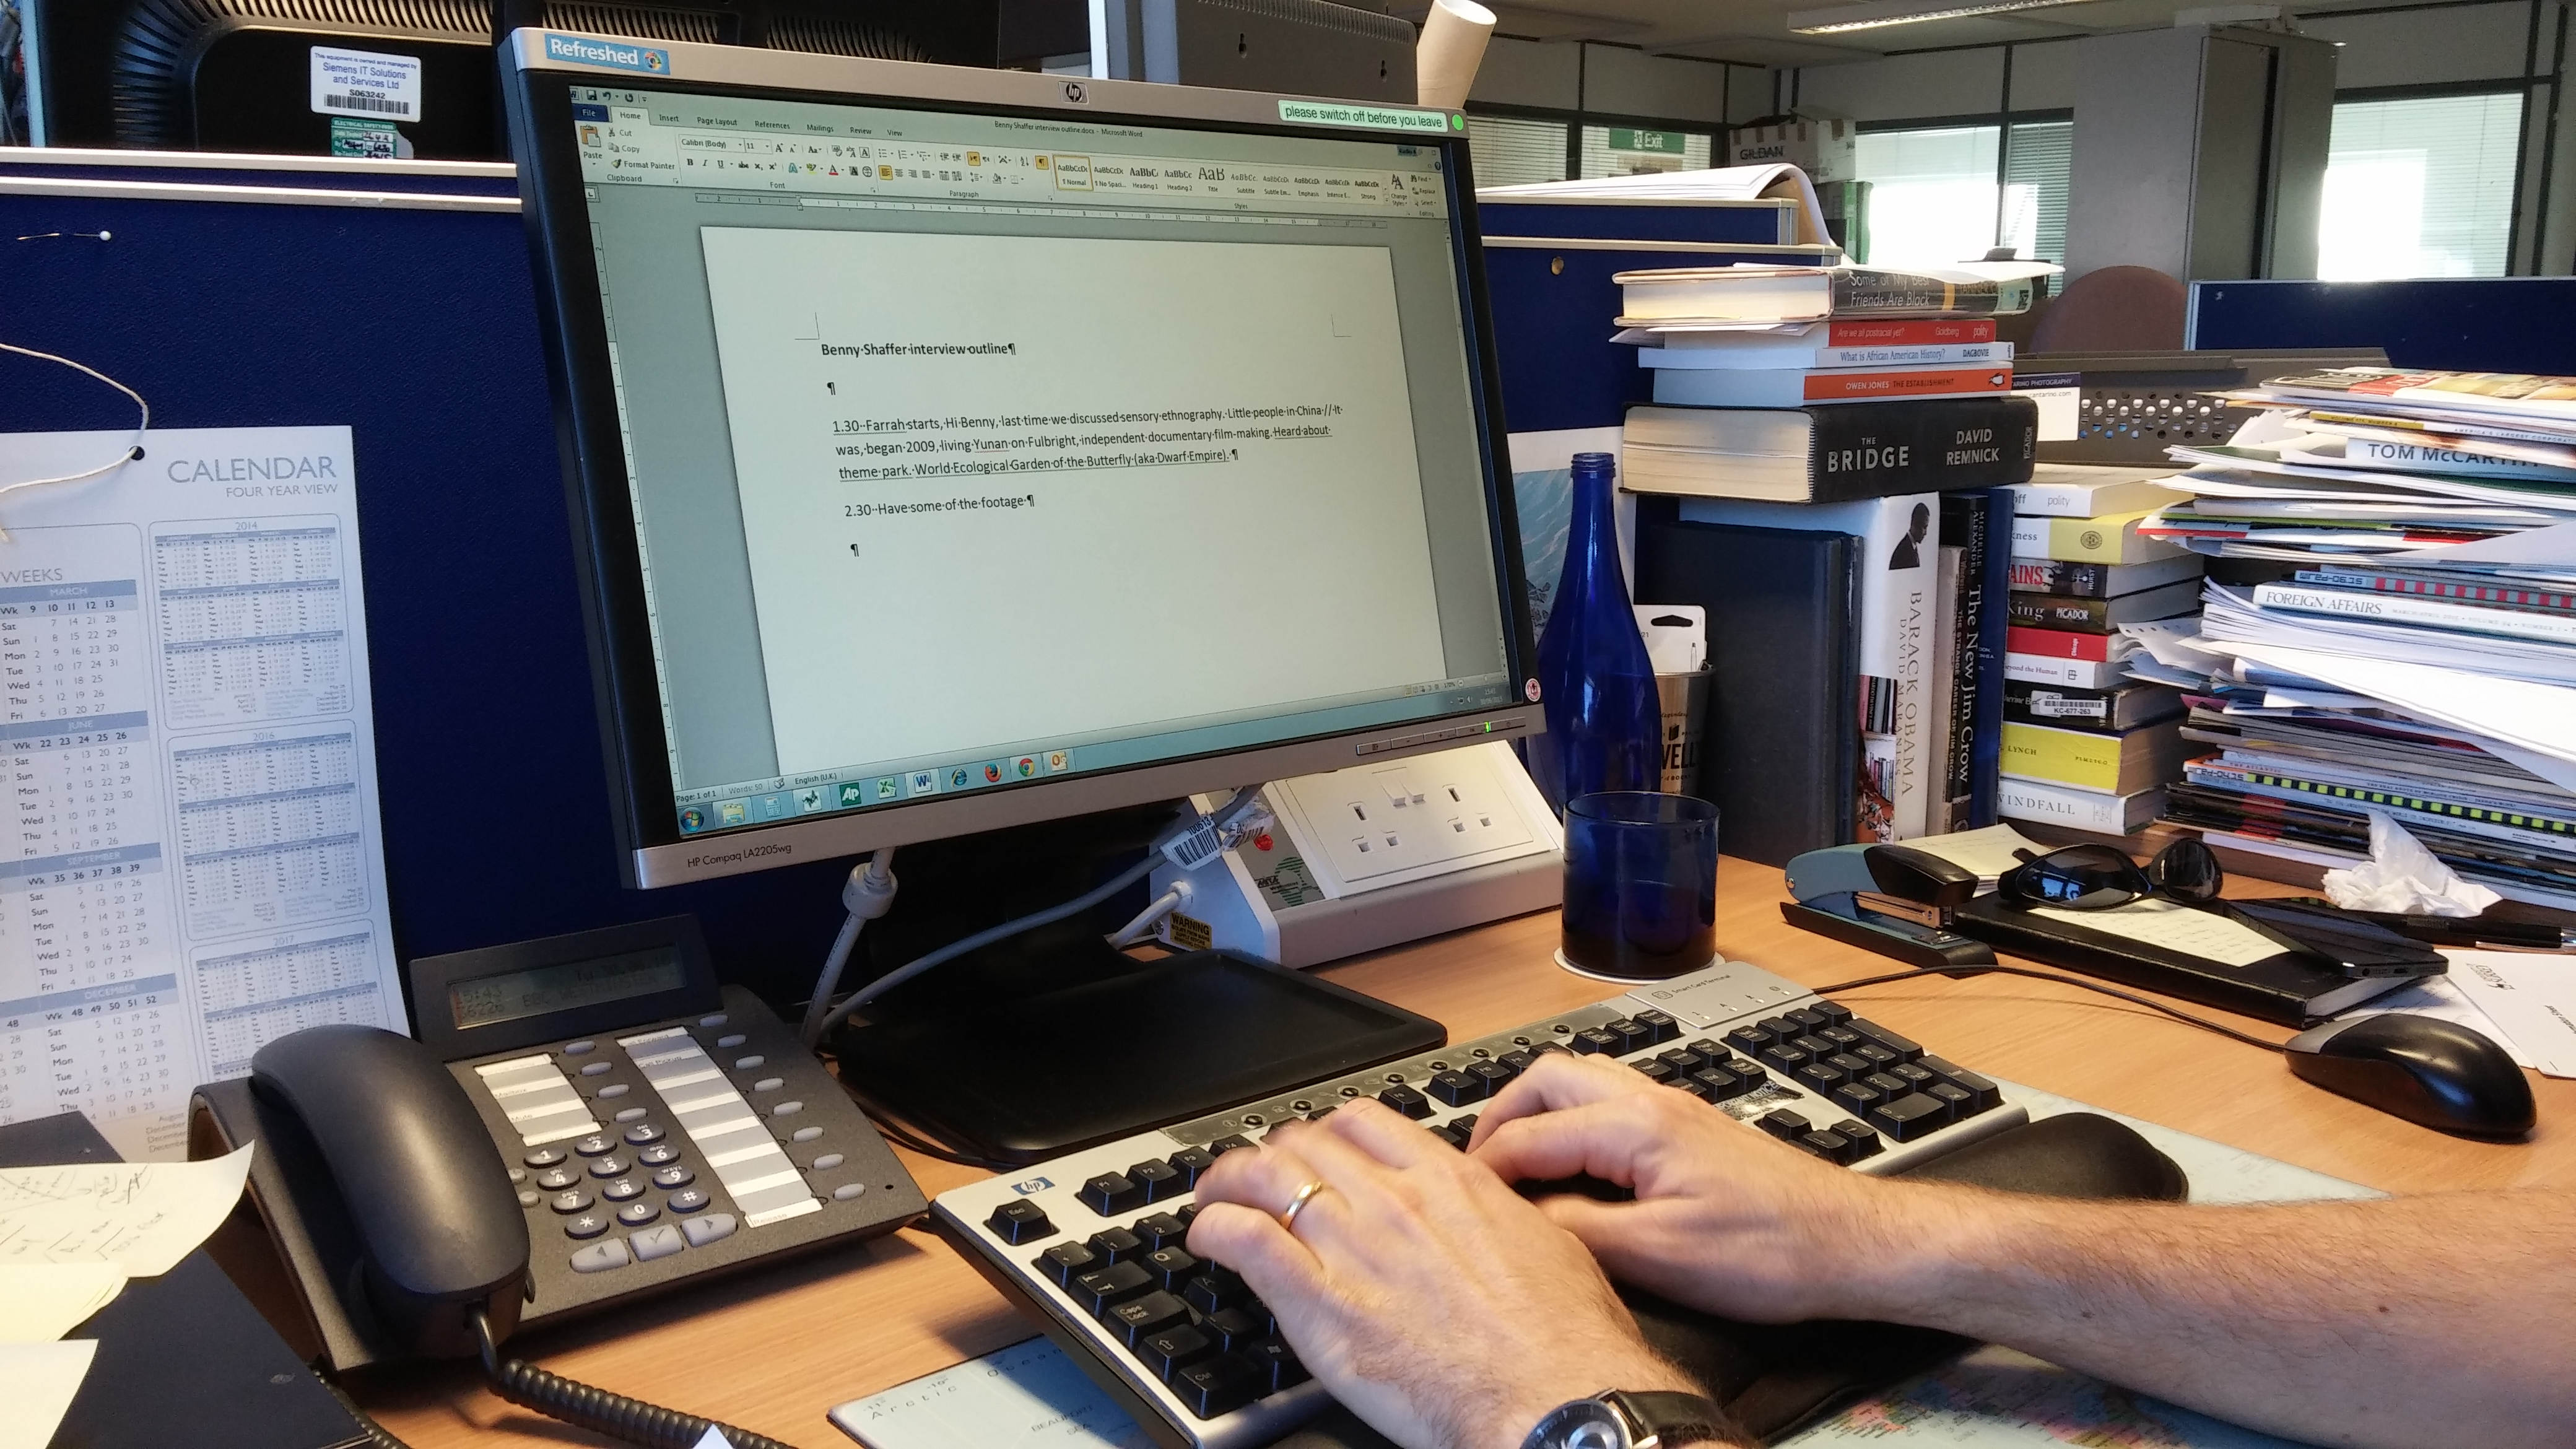
\includegraphics[width=0.6\textwidth]{figs/study2-participantA-workspace.jpg}
  \caption{Work environment}
  \label{fig:study2-participantA-workspace}
\end{figure}

----

Speech editor prototupe
42 min interview
==> start making notes 15.58
correcting words
moved to word
copied into word
marking paragraphs using start ratings and notes at end of paragraph
paragraphs separated using speaker diarization
skim reads as was there at the recording
6700 words from transcript
"[**** should use this Homer stuff, but dramatically cut down]"
bold lots of sentences
"[***** this is the point of the whole show]"
==> 3 min phone call
==> finished making notes 16.16
- bold, italic, underline options
==> start cutting 16.20
select and cut out individual pieces
would be useful to name downloaded wav
needed to zoom way out to fit long (5 minute) edit
not using search feature, just scrolling and matching to bold highlighted word
file
==> finished cutting 16.28
asked for search - wasn't obvious to use browser
ability to make and search annotations

Speaker diarization (implicit)
Fast forward / speed up

TLX metrics:
Mental demand: -1
Physical demand: -7
Temporal demand: -6
Performance: -7
Effort: +2
Frustration: -8

\subsubsection{Participant B}

Old method:
interview 15.5 minutes in durationusing FCP on Macbook Air (11" screen) - as normal desktop does not have it installed
?? WHY USE FCP INSTEAD OF BBC SUPPORTED SOFTWARE?
using trackpad
problems with connecting hard drive
backups in Box.com
==> opened software 12.25
creates new library
creates new project
==> project created 12.26
import media
==> media imported 12.27
uses keyboard shortcuts to naviagate in asset section of interface
?? LISTENING DOUBLE SPEED? CHIPMUNK STYLE?
puts 'placeholder' in timeline
?? WHAT IS PLACEHOLDER IN TIMELINE?
listens through press M for mark
?? WHAT DOES MARK REPRESENT?
?? HOW MANY MARKS MADE?
after going through one-third of the interview, goes back using markers to create in and out points and put in timeline
FCP displays energy plot
goes back to chop up after two-thirds the way through
=> finished going through at 12.41
6 clips pulled out, now down to ~9 mins
marks represent good points/phrases, crowding of markers is good
markers are a rating system of sorts
trouble finding title feature in menus
drops in title, gives name of interview, stretch to length of all interview clips
called 'sync pull'
won't go back to rushes
will make new project for programme assembly
export programme assembly as stereo wav, then import into SADiE
export and import process takes about  5 mins
then chop and name clips, takes 15-20 mins for 45 programme
titles is useful feature
FCP can process and improve audio on import (e.g. very different levels, low levels) as tick box on import process
includes library of SFX as standard, not used very often

TLX metrics:
Mental: +5.5
Physical: -0.5
Temporal: -2.5
Performance: -5.5
Effort: +5.5
Frustration: +2.5

\begin{figure}[ht]
  \centering
  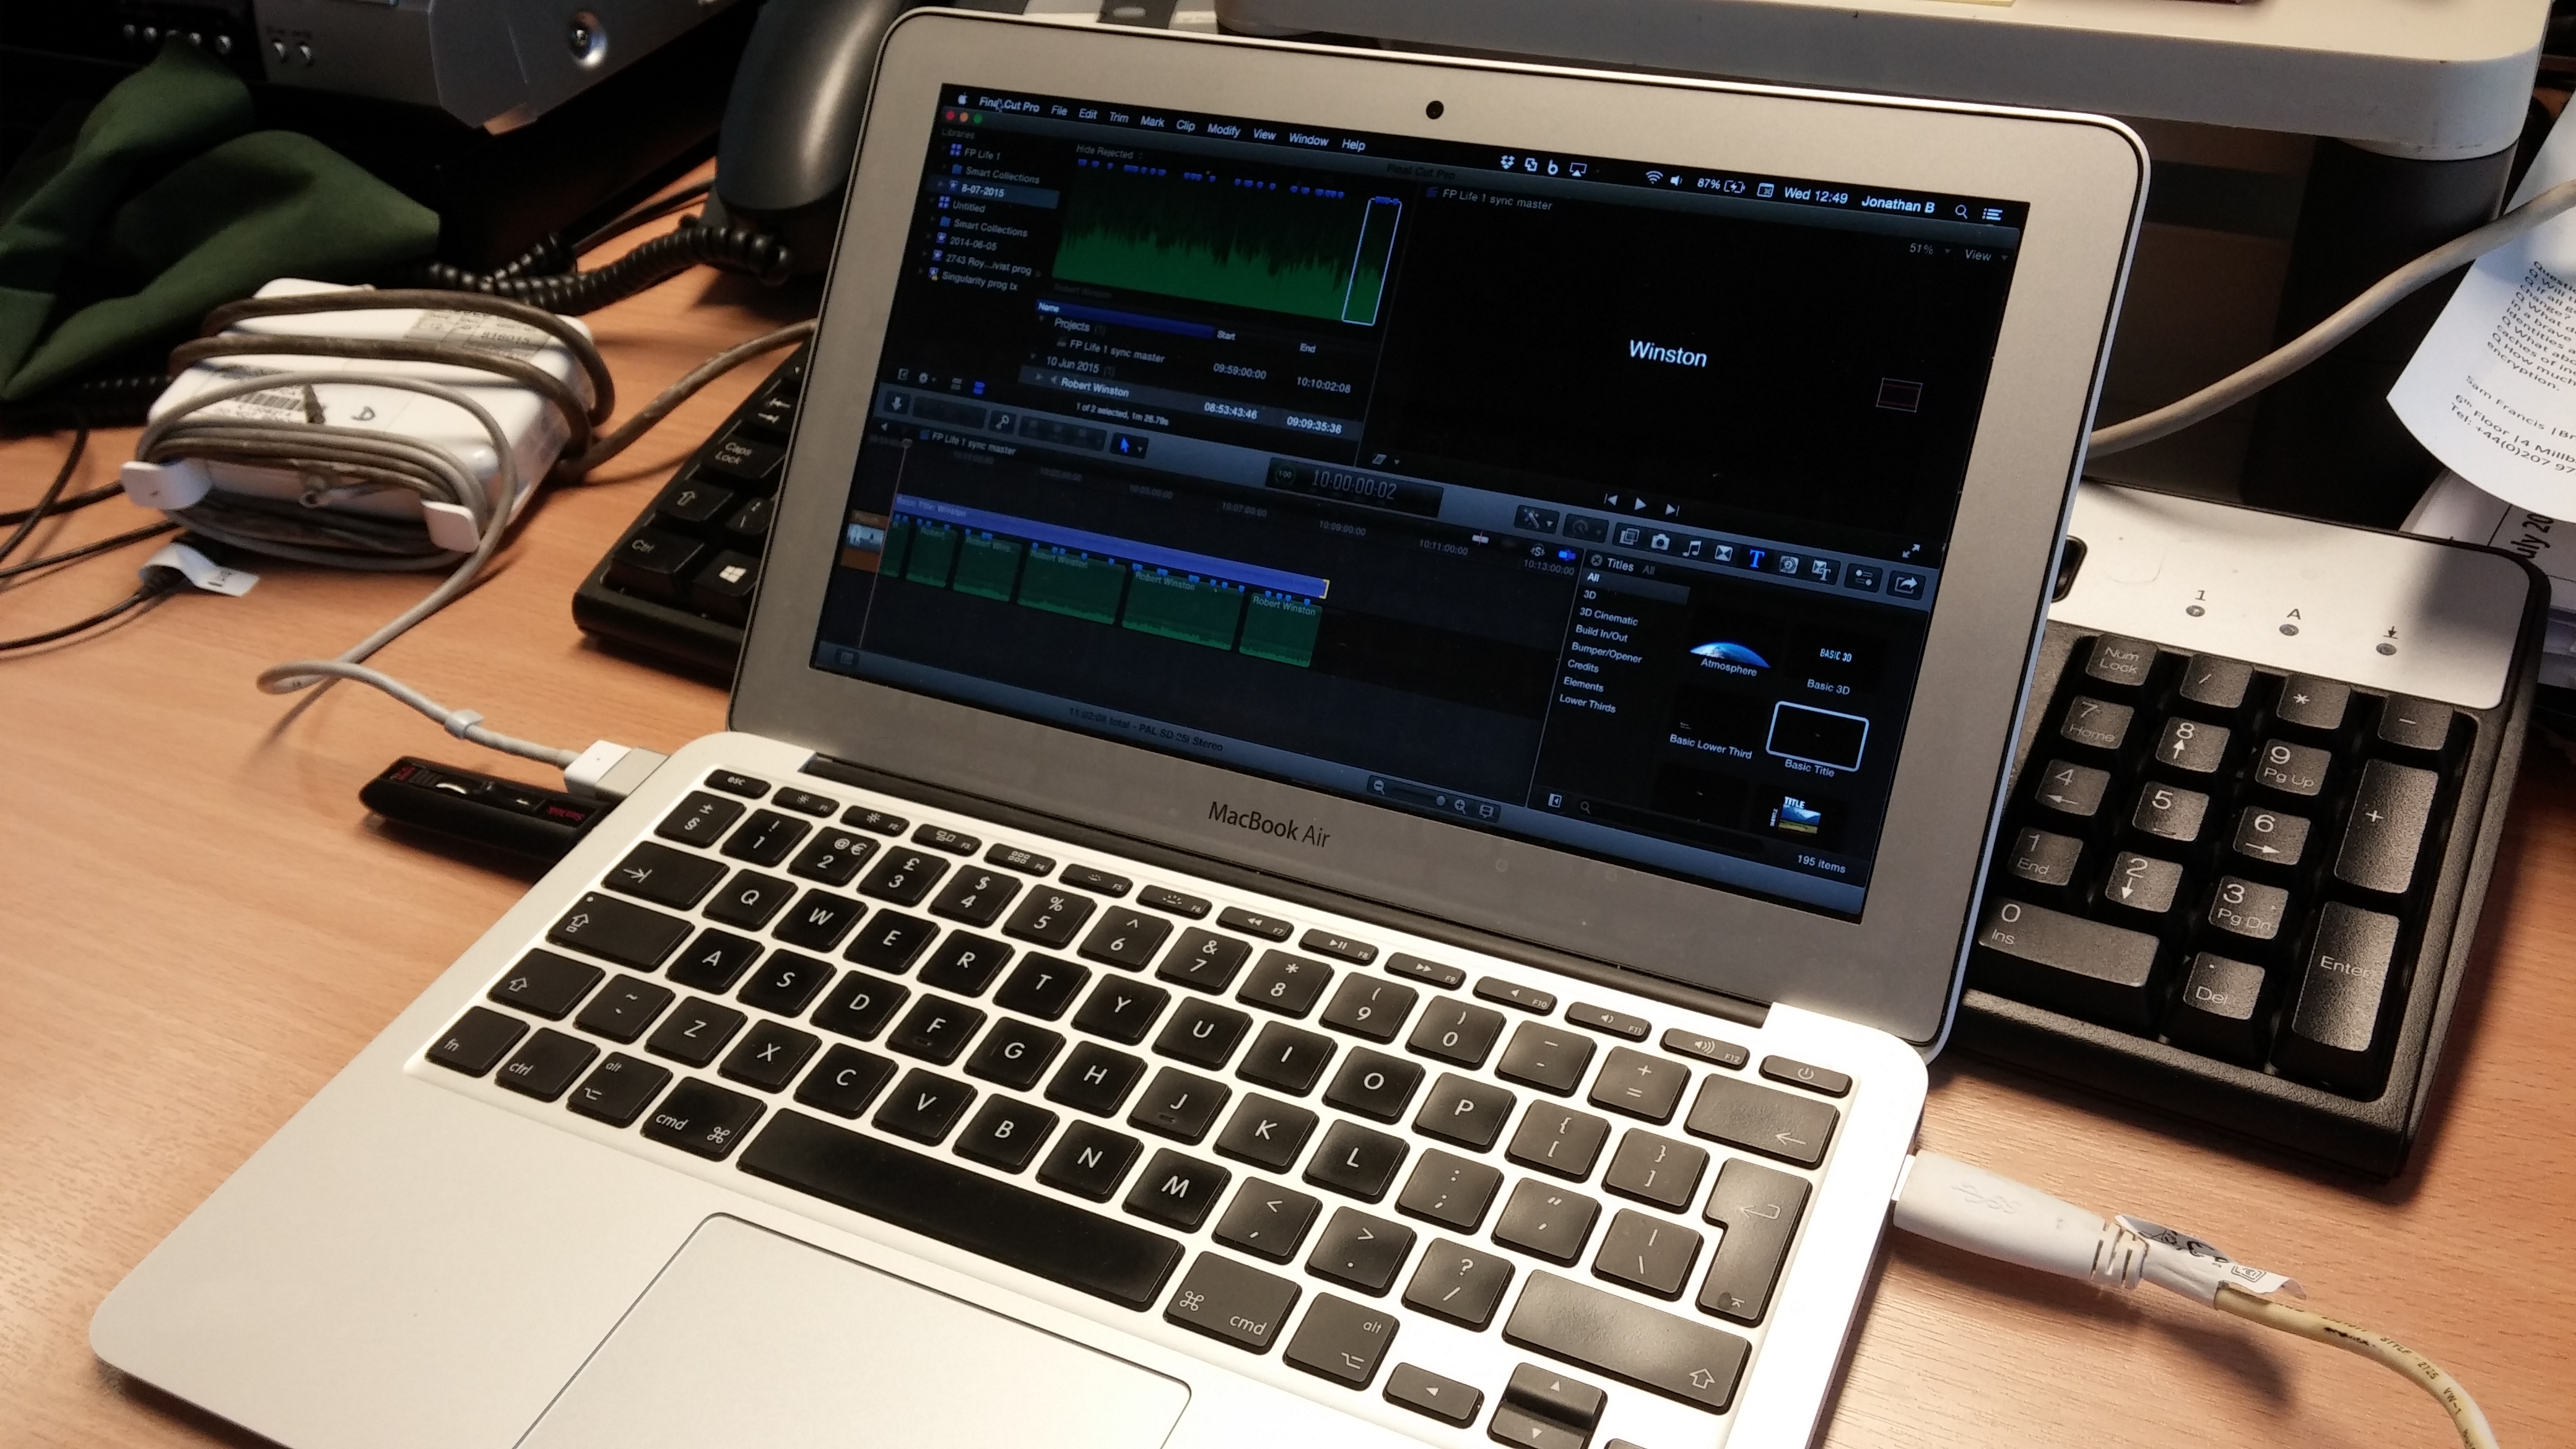
\includegraphics[width=0.6\textwidth]{figs/study2-participantB-workspace.jpg}
  \caption{Work environment}
  \label{fig:study2-participantB-workspace}
\end{figure}

New method
34 min interview
==> Opened software 12.53
print transcript immediately
==> print command sent 12.54
?? WHY CHOOSE TO PRINT?
==> paper in hand 12.56
using highlighter pen
?? IS TRANSCRIPT GOOD ENOUGH?
?? PAGE NUMBERS?
no page numbers or timestamps
?? WOULD STILL USE PAPER IF ANNOTATION FEATURES IN SOFTWARE?
highlighting full lines, not down side
sometimes highlights ocassional sentence in long paragraph, sometimes highlights almost all of paragraph, minus some short bits
?? RECALLING ORIGINAL INTERVIEW?
?? MISS NOT HAVING THE AUDIO?
?? READING EVERYTHING OR TRYING TO FIND BITS REMEMBERED?
?? SPEAKER DIARIZATION USEFUL? ALREADY ANNOTATED? HOW DONE? HOW LONG?
==> finished highlighting paper at 13.12
==> started editing on screen at 13.14
used ctrl+F to find highlighted bits from paper (five times in total), chooses to search for rare words
need to select in and out points by matching text between paper and screen
needed to drop big paragraph in middle then rearrange others to put at bottom, forgot to move one to bottom
told about zoom in/out, which was used to zoom out
when short words or phrases weren't highlighted, chose to include them in a larger selection
when zoomed out, rearranging doesn't make sufficient gaps
expressed annoyment at not having enough space to put more clips when full
scrollbar could be bigger (especially when zoomed out)
accidentally highlights everything in stage sometimes (preventable)
could make draggable more transparent to see rearrangement, user was moving draggable to side so they could see
==> finished editing on screen at 13.30
edited down to 10 mins
two choices now - export WAV then import into FCP, identify gaps, add spaces, add title (probably 10-15 mins to do spacing) what he would probably do without SADiE option, OR import into SADiE directly
==> imported into SADiE at 13.36
presenter is on right channel, contributor on left
wants to start putting gaps in
noted that nothing has been listened to, some bits don't sound as good as words make it out to be, could try and tidy up or find better bits
wants to listen through to everything to see if it can be chopped further based on how it sounds (at double speed)
this edit is more 'edisodic' than the first interview in which he's looking for short bits to use throughout doc
wouldn't want to use transcript to further reduce rough edit
wouldn't use transcription interface as (a) its an extra redundant process (b) no way to speed up playback speed (c) SADiE is more flexible and powerful (d) music can be added
can't mix with different rough edits
?? MIXING ROUGH EDITS IN INTERFACE, WHAT IS PREVENTING
wants to highlight and hit a key - drag and drop only used for reordering
butt joining clips makes less sense as they jump around
15 clips made
interface not accessible offline - another reason for using paper

TLX metrics:
Mental: -2.5
Physical: +2.5
Temporal: +0.5
Performance: +0.5
Effort: -0.5
Frustration: +3.5

\begin{figure}[ht]
  \centering
  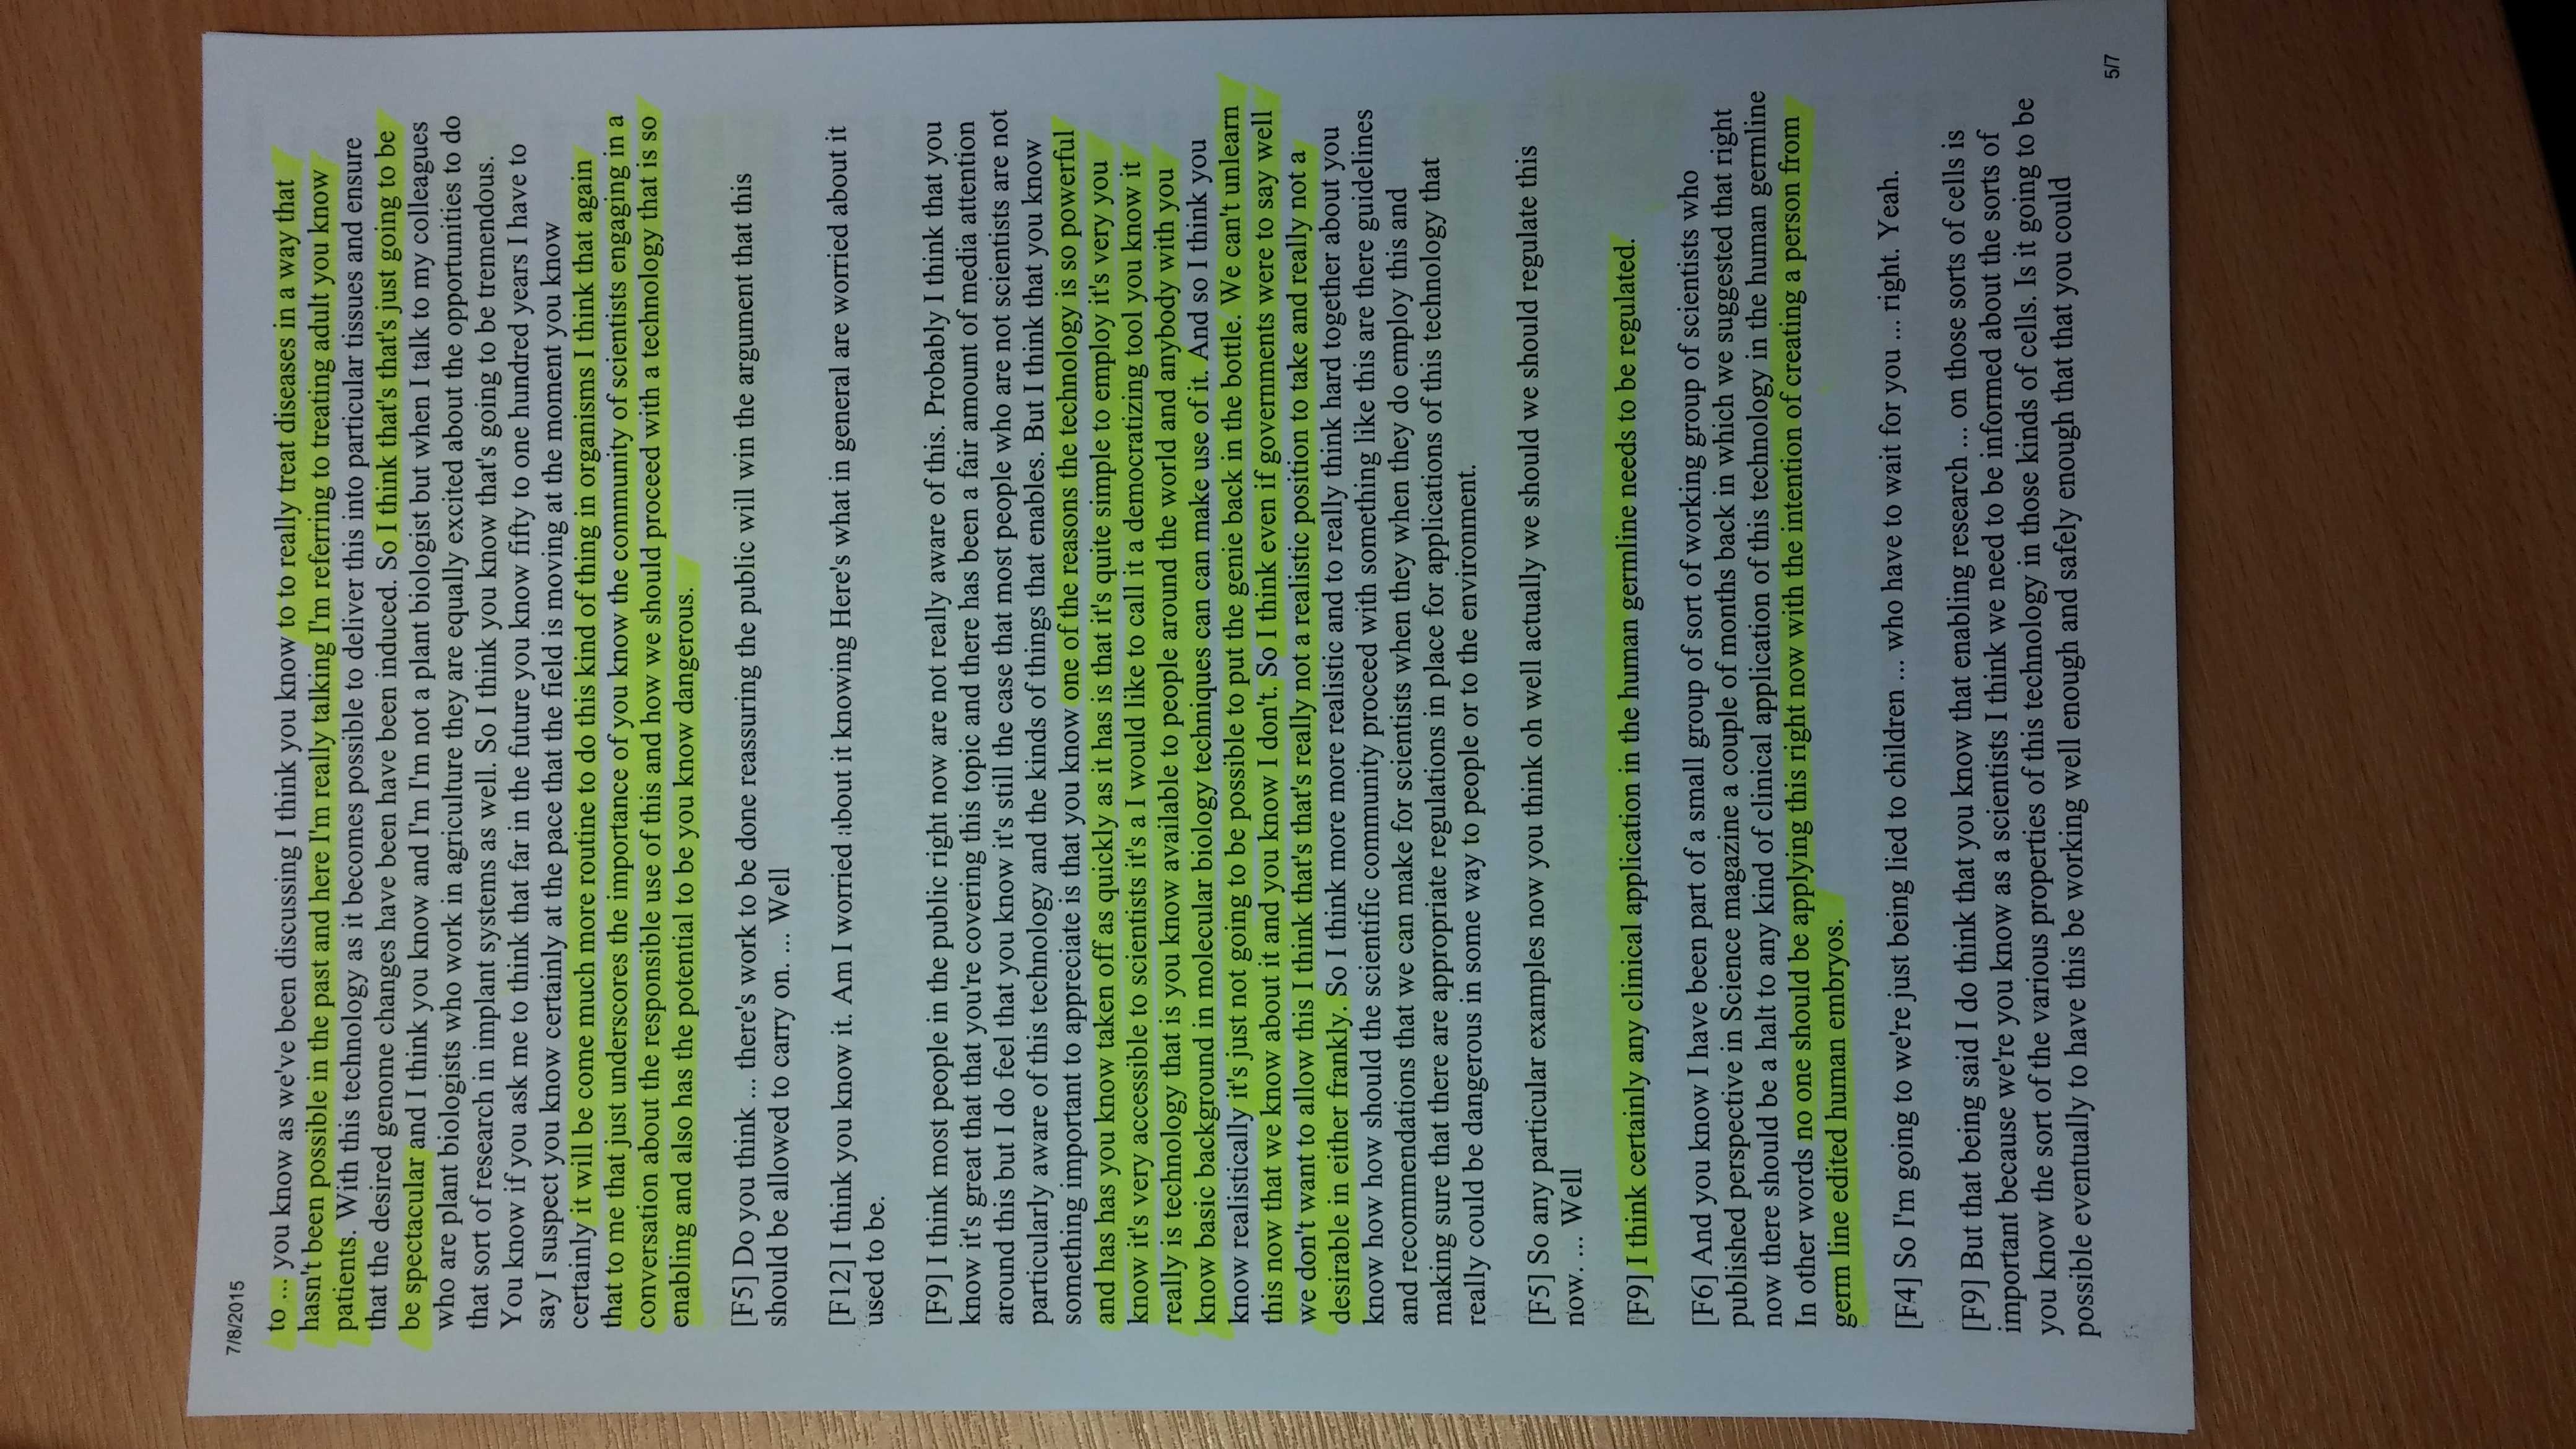
\includegraphics[width=0.6\textwidth]{figs/study2-participantB-printout.jpg}
  \caption{Transcript annotation}
  \label{fig:study2-participantB-printout}
\end{figure}

---
?? USEFUL/ NOT USEFUL BITS
?? CHANGE WORKFLOW
?? WHICH METHOD PREFERRED? WHY?
?? THINGS TO IMPROVE?
?? PREFER READING OR DOUBLE SPEED LISTENING?
?? PREFER PAPER OR SCREEN? WHY?
?? DO THINGS THE SAME WAY NEXT TIME?

